\documentclass[12pt]{article}

\usepackage{amsmath}
\usepackage{amssymb}
\usepackage{anyfontsize}
\usepackage[toc,page]{appendix}
\usepackage{array}
\usepackage{authblk}
% \usepackage{background}
\usepackage{booktabs}
\usepackage{caption}
\usepackage{cellspace}
\usepackage{color}
\usepackage{enumerate}
\usepackage{enumitem}
\usepackage{fancyhdr}
\usepackage{float}
\usepackage{fontspec}
\usepackage{geometry}
\usepackage{graphicx}
\usepackage{listings}
\usepackage{multicol}
\usepackage{physics} 
\usepackage{sectsty}
\usepackage{subfigure}
\usepackage{unicode-math}
\usepackage{url}
\usepackage{tabularx}
\usepackage{wallpaper}
\usepackage{xeCJK}

\setmainfont{Times New Roman}
\setCJKmainfont{教育部標準宋體UN}
\setmonofont{Courier New}
\setmathfont{XITS Math}

\renewcommand\thesection{\Roman{section}.}
\renewcommand\thesubsection{\normalsize\roman{subsection}.}
\sectionfont{\centering\large}
\subsectionfont{\centering\normalsize\it}

\geometry{
    a4paper,
    total = {170mm, 257mm},
    left = 20mm,
    top = 20mm,
    }
    
% \backgroundsetup{
%                 firstpage = false,   
%                 angle   = 0,
%                 opacity = 1,
%                 scale   = 1,
%                 placement = bottom,
%                 contents={
%                          
\includegraphics[width=50mm]{../figure/nthu-logo.png}
%                             },
%                 position={140mm, 8mm},
%                     }

\setlength{\unitlength}{1mm}
% \setlength{\headheight}{5mm}

\definecolor{dkgreen}{rgb}{0,0.6,0}
\definecolor{gray}{rgb}{0.5,0.5,0.5}
\definecolor{mauve}{rgb}{0.58,0,0.82}
\lstset{frame = tb,
        language = Python,
        aboveskip = 3mm,
        belowskip = 3mm,
        showstringspaces = False,
        columns = flexible,
        basicstyle = {\small\ttfamily},
        numbers = left,
        numberstyle = \tiny\color{gray},
        keywordstyle = \color{blue},
        commentstyle = \color{dkgreen},
        stringstyle = \color{mauve},
        breaklines = true,
        breakatwhitespace = true,
        tabsize = 4}


%%%%%%%%%%%%%%%%%%%%%%%%%%%%%%%%%%%%%%%%%%%%%%% Again, Don't change anything Above %%%%%%%%%%%%%%%%%%%%%%%%%%%%%%%%%%%%%%%%%%%%%%%


\begin{document}

\pagestyle{fancy}
    \fancyhf{} % clear all header and footer fields
    \renewcommand{\headrulewidth}{0pt} %clear the header line 
    \fancyhead[R]{
        \ifnum\value{page}>1 
            \begin{picture}(170, 257)
                \put(120,247){\hbox{
\includegraphics[width=50mm]{../figure/nthu-logo.png}}}
            \end{picture}
        \else \fi
        }
    \fancyfoot[C]{\thepage}

% title and info
\title{{\vspace{-2.5cm}
        \normalsize Collider Physics - Final Report}\\
        \textbf{Atmospheric Neutrino Oscillation in Super-K}}
\author{Yuan-Yen Peng(彭元彥)}
\affil{ \it{Dept. of Physics, NTHU}\\
        \it{Hsinchu, Taiwan}}
\date{\today}
\maketitle

\setlength{\columnsep}{0.03\textwidth}
\begin{multicols}{2}
\thispagestyle{fancy}

\section{Neutrino}
    Four types of neutrino sources can be classified into solar neutrinos, atmospheric neutrinos, accelerator neutrinos, and reactor neutrinos. Additionally, these neutrino sources are investigated in different experimental facilities. As the aforementioned, the first affiliated neutrino observatory is SNO (Sudbury Neutrino Observatory) in Canada; the second representative neutrino observatory is Super-K (Super Kamiokande) in Japan; the third corresponding observatories are KEK-SuperK (Japan), T2K (Japan), etc; the last observatories representing are KamLAND (Japan), Daya bay (China), etc. In this final report, we are going to present and elaborate on atmospheric neutrino oscillation in Super-K.

    \subsection{Neutrino Oscillation}
        Neutrino oscillation is a phenomenon that describes the flavor of neutrino oscillating among three different flavors; further, this phenomenon can explain the existence of neutrino mass (i.e., $\Delta m$). In general, the ``flavor eigenstates'' are related to the ``mass eigenstates'' with the $3 \times 3$ unitary mixing matrix:
        \[
            | \nu_{\alpha} \rangle = \sum_{i} U_{\alpha i} | \nu_{i} \rangle
        \]
        The matrix $U$ is the PMNS matrix (Pontecorvo-Maki-Nakagawa-Sakata matrix: mixing flavor eigenstates of leptons); $\nu_\alpha$ is the mass eigenstate and $\nu_i$ is the flavor eigenstate. Thus, we need the PMNS matrix in order to find the relation between eigenspaces. The PMNS matrix is \cite{SKexp} \cite{AtoNeu}:
        \begin{align*}
            U_{\alpha i} &= 
            \begin{bmatrix}
                U_{e1}     & U_{e2}     & U_{e3}    \\
                U_{\mu 1}  & U_{\mu 2}  & U_{\mu 3} \\
                U_{\tau 1} & U_{\tau 2} & U_{\tau 3}\\
            \end{bmatrix}\\
            &=
            \begin{bmatrix}
                1 & 0       & 0     \\
                0 & c_{23}  & s_{23}\\
                0 & -s_{23} & c_{23}\\
            \end{bmatrix}
            \times
            \begin{bmatrix}
                c_{13}             & 0 & s_{13}e^{i\delta}\\
                0                  & 1 & 0                \\
                -s_{13}e^{i\delta} & 0 & c_{13}           \\
            \end{bmatrix}\\
            &\quad \mathbin \times
            \begin{bmatrix}
                c_{12}  & s_{12} & 0\\
                -s_{12} & c_{12} & 0\\
                0       & 0      & 1\\
            \end{bmatrix}
        \end{align*}
        where $\alpha = e,\ \mu,\ \tau$; $i = 1,\ 2,\ 3$; $c_{ab}$ and $s_{ab}$ means $sin$ and $cos$ with mixing angle $\theta_{ab}$; $\delta$ means CP-violating phase (s.t. second term of the matrix is small). The first term of the matrix is corresponding to ``solar mixing'', the second term of the matrix is known to be small, and the third term of the matrix describes ``atmospheric mixing''.

        The experiment of testing the neutrino oscillation needs a distance $L$ to let neutrinos propagate. We, thence, need to investigate the state propagation. For mass eigenstate 
        \[
            |\nu_{j}(t)\rangle = e^{-i(E_{j}t - \vec{p_{j}} \cdot \vec{x})} |\nu_{j}(0)\rangle
        \]
        take ultrarelativistic limit $|\vec{p_j}| \gg m_j$ and also drop out the relative phase. When $t\approx L$ \cite{AtoNeu}: 
        \begin{align*}
            E_{j}           &= \sqrt{\mathbf{p_{j}}^{2} + m_{j}^{2}} = \mathbf{p_{j}}\sqrt{1 + \frac{m_{j}^{2}}{\mathbf{{p}_{j}^{2}}}}\\
                            &\approx \mathbf{p_{j}} \big( 1 + \frac{m_{j}^{2}}{2 \mathbf{p_{j}^{2}}} \big) = \mathbf{p_{j}} + \frac{m_{j}^{2}}{2 \mathbf{p_{j}}}\\
            \Delta E_{ij}   &= \Big( \mathbf{p_{i}} + \frac{m_{i}^{2}}{2 \mathbf{p_{i}}} \Big) - \Big( \mathbf{p_{j}} + \frac{m_{j}^{2}}{2 \mathbf{p_{j}}} \Big) = \frac{\Delta m_{ij}^{2}}{2E} 
        \end{align*}
        Considering the difference of the state and taking the above approximation (here, we use $ij$ to indicate the difference, but in the following equation (\ref{prob_raw}) we use $jk$ to avoid garbling with imaginary), we can get:
        \[
            |\nu_{ij}(L)\rangle = e^{-i(\frac{\Delta m_{ij}^{2}L}{2E})} |\nu_{ij}(0)\rangle
        \]

        In the wake of knowing the propagation of the mass eigenstate, we want to know the ``interference'' between the flavor eigenstates. Therefore, we suppose the initial lepton with the flavor eigenstate $\alpha$ and desire to know what is the ``probability'' if observing the flavor eigenstate $\beta$ when $t \approx L$ is \cite{SKexp}:
        \begin{align*}
            P_{\alpha \rightarrow \beta}&= |\langle\nu_{\beta}|\nu_{\alpha}\rangle|^{2}\\
                                        &= \Big| \sum_{j}U_{\alpha j}^{*}U_{\beta j}e^{-i(\frac{m_{j}^{2}L}{2E})} \Big|^2\\
                                        &\qquad \text{drop out}\ \mathbb{Im}\\
                                        &\begin{aligned}[c]
                                            \Rightarrow \delta_{\alpha \beta}   &- 4\sum_{j > k} \mathbb{Re} \Bigl\{ U_{\alpha j}^{*}U_  {\beta j}U_{\alpha k}U_{\beta k}^{*} \Bigr\}\\ 
                                                                                &\mathrel \times \sin^{2} \Big( \frac{\Delta_{jk}m^2L}{4E} \Big)
                                        \end{aligned}
                                        \tag{I}\label{prob_raw}
        \end{align*}
    
        \subsection{One mass scale dominant approximation}
        The one mass scale dominant approximation means there is one mass among the three masses which is manifest larger than the others in the mass square difference. (This approximation has been supported by the neutrino experiments \cite{SKexp}) Here, we suppose $m_3$ is the dominant mass :
        \[
            \big| m_{2}^{2} - m_{1}^{2} \big| \ll \big| m_{3}^{2} - m_{1,2}^{2} \big|
        \]
        Moreover, we can rewrite the phase inside the square of $\sin$ in equation (\ref{prob_raw}) as:
        \begin{align*}
            \frac{\Delta_{jk}(mc)_{2}L}{4 \hbar c} &= \frac{GeV\ fm}{4 \hbar c} \times \frac{\Delta_{jk} m^2}{eV^2} \frac{L}{km} \frac{GeV}{E}\\
            &\approx 1.27 \times \frac{\Delta_{jk} m^2}{eV^2} \frac{L}{km} \frac{GeV}{E}
        \end{align*}
        According to this method, the propagating probabilities in vacuum for atmospheric neutrinos are \cite{SKexp} : 
        \begin{align*}
                P(\nu_{e} \rightarrow \nu_{\mu})    &= P(\nu_{\mu}\rightarrow \nu_{e})\\
                                                    &= \sin^{2}\theta_{23} \sin^{2} 2\theta_{13} \sin^{2}\Big( \frac{1.27 \Delta m^{2} L}{E} \Big) \tag{II}\label{prob} \\
                P(\nu_{e} \rightarrow \nu_{e})      &= 1 - \sin^{2} 2\theta_{13}\sin^{2} \sin^{2}\Big( \frac{1.27\Delta m^{2} L}{E} \Big)\\ 
                P(\nu_{\mu} \rightarrow \nu_{\mu})  &= \begin{aligned}[t]
                                                            1 - &4 \cos^{2}\theta_{13}\sin^{2}\theta_{23}\\
                                                                &\times \big( 1 - \cos^{2}\theta_{13}\sin^{2} \theta_{23} \big)\\
                                                                &\times \sin^{2}\Big( \frac{1.27\Delta m^{2} L}{E} \Big)\\
                                                        \end{aligned}
        \end{align*}
        Here, we consider that neutrinos propagate in constant matter Earth density \cite{SKexp}, so equation (\ref{prob}) will become:
        \begin{align*}
            P(\nu_{e} \rightarrow \nu_{\mu})    &= P(\nu_{\mu}\rightarrow \nu_{e})\\
                                                &= \sin^{2} \theta_{23} \sin^{2} 2\theta_{13}^{M} \sin^{2}\Big( \frac{1.27 \Delta m^{2} L}{E} \Big)\\
        \end{align*}
        where, the effective mixing angle $\theta^{M}$ is defined as:
        \[
            \sin^{2}2\theta_{13}^{M} = \frac{\sin^{2}2\theta_{13}}{(\cos2\theta_{13} - A_{CC}/\Delta m^{2})^{2} + \sin^{2}2\theta_{13}}
        \]
        The matter potential term is $A_{CC} = 2\sqrt{2}G_{F}N_{e}p$, where $G_{F}$, $N_{e}$ and $p$ are Fermi constant, electron density, and neutrino momentum, respectively.

    \subsection{Two states oscillation}
        Considering the probabilities functions obtained in the aforementioned, we can take a limit of infinitesimal $\theta_{13}$, it will only allow neutrino oscillating between flavors of $\tau$ and $\mu$; i.e, two flavor states oscillation, also we can see the probabilities of different initial neutrino oscillating to others in Figure \ref{NeuOsci}. Hence, we can reduce the probability function as:
        \[
            P_{\alpha \rightarrow \beta} = \sin^{2} 2\theta \sin^{2} \Big( \frac{1.27 \Delta m^{2}L}{E} \Big)\ \Big[ \text{Natural Units} \Big]
        \] 
        \begin{figure}[H]
            \centering 
            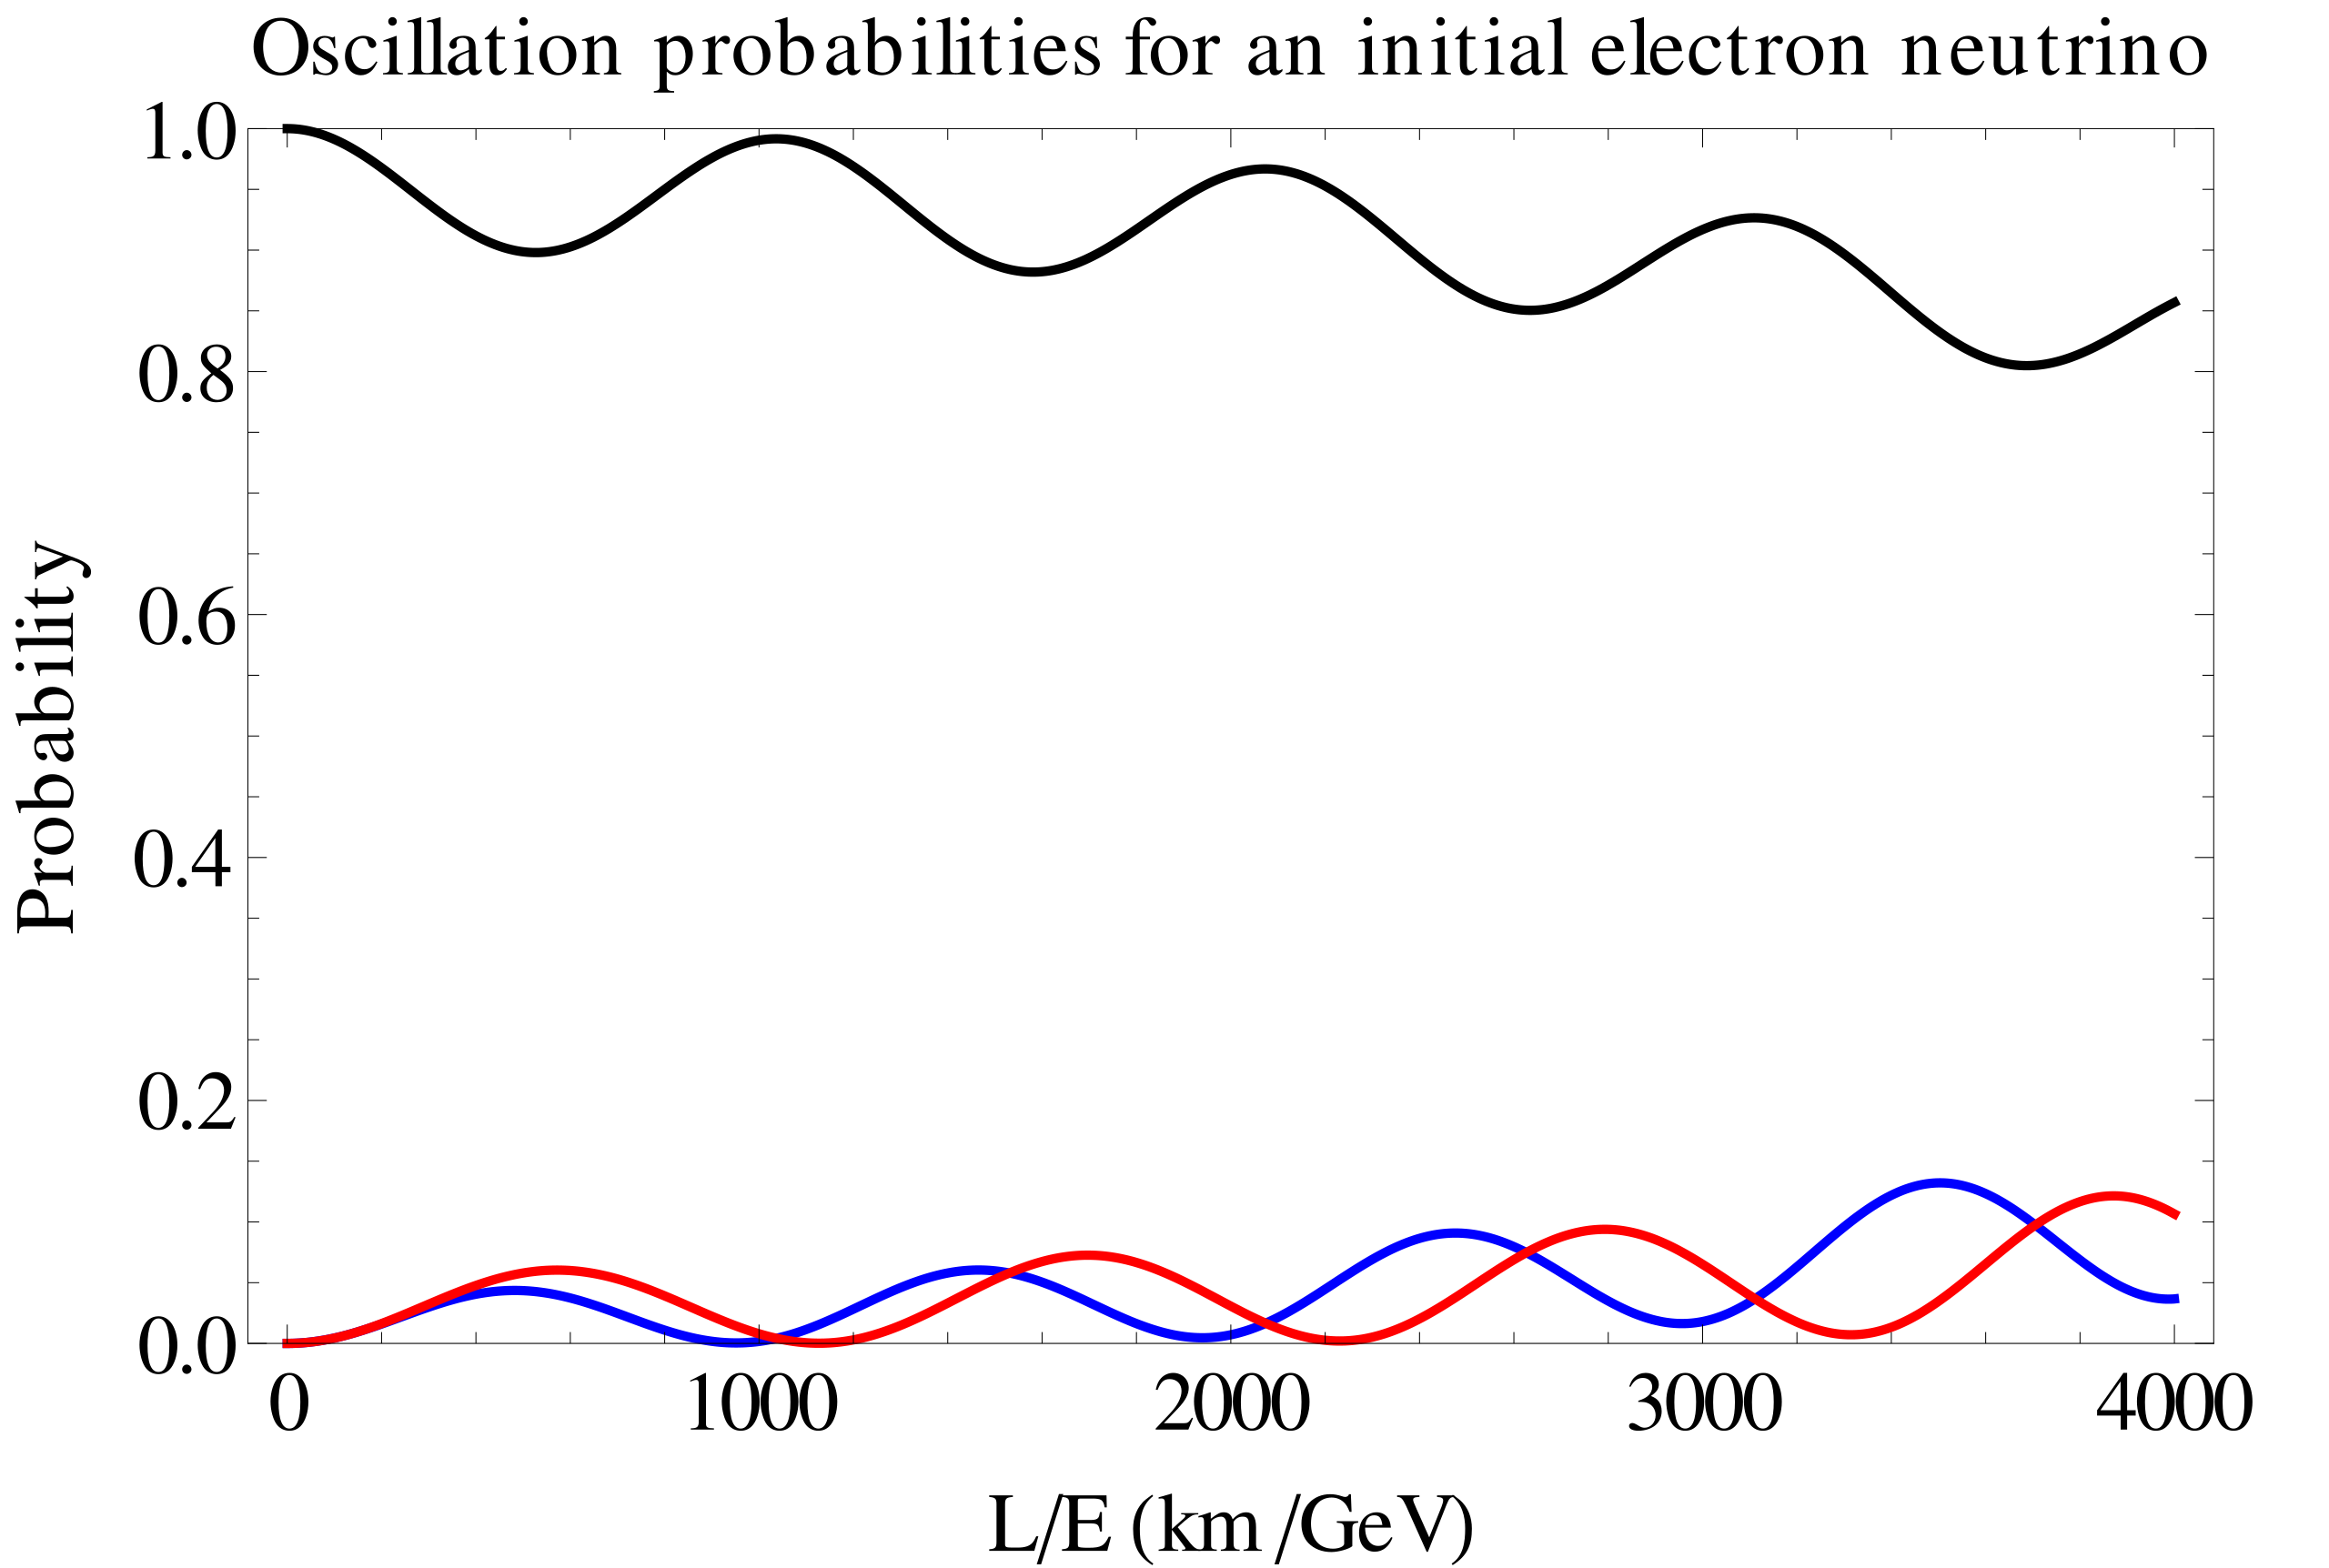
\includegraphics[width = 0.45\textwidth]{../figure/e.png}  
            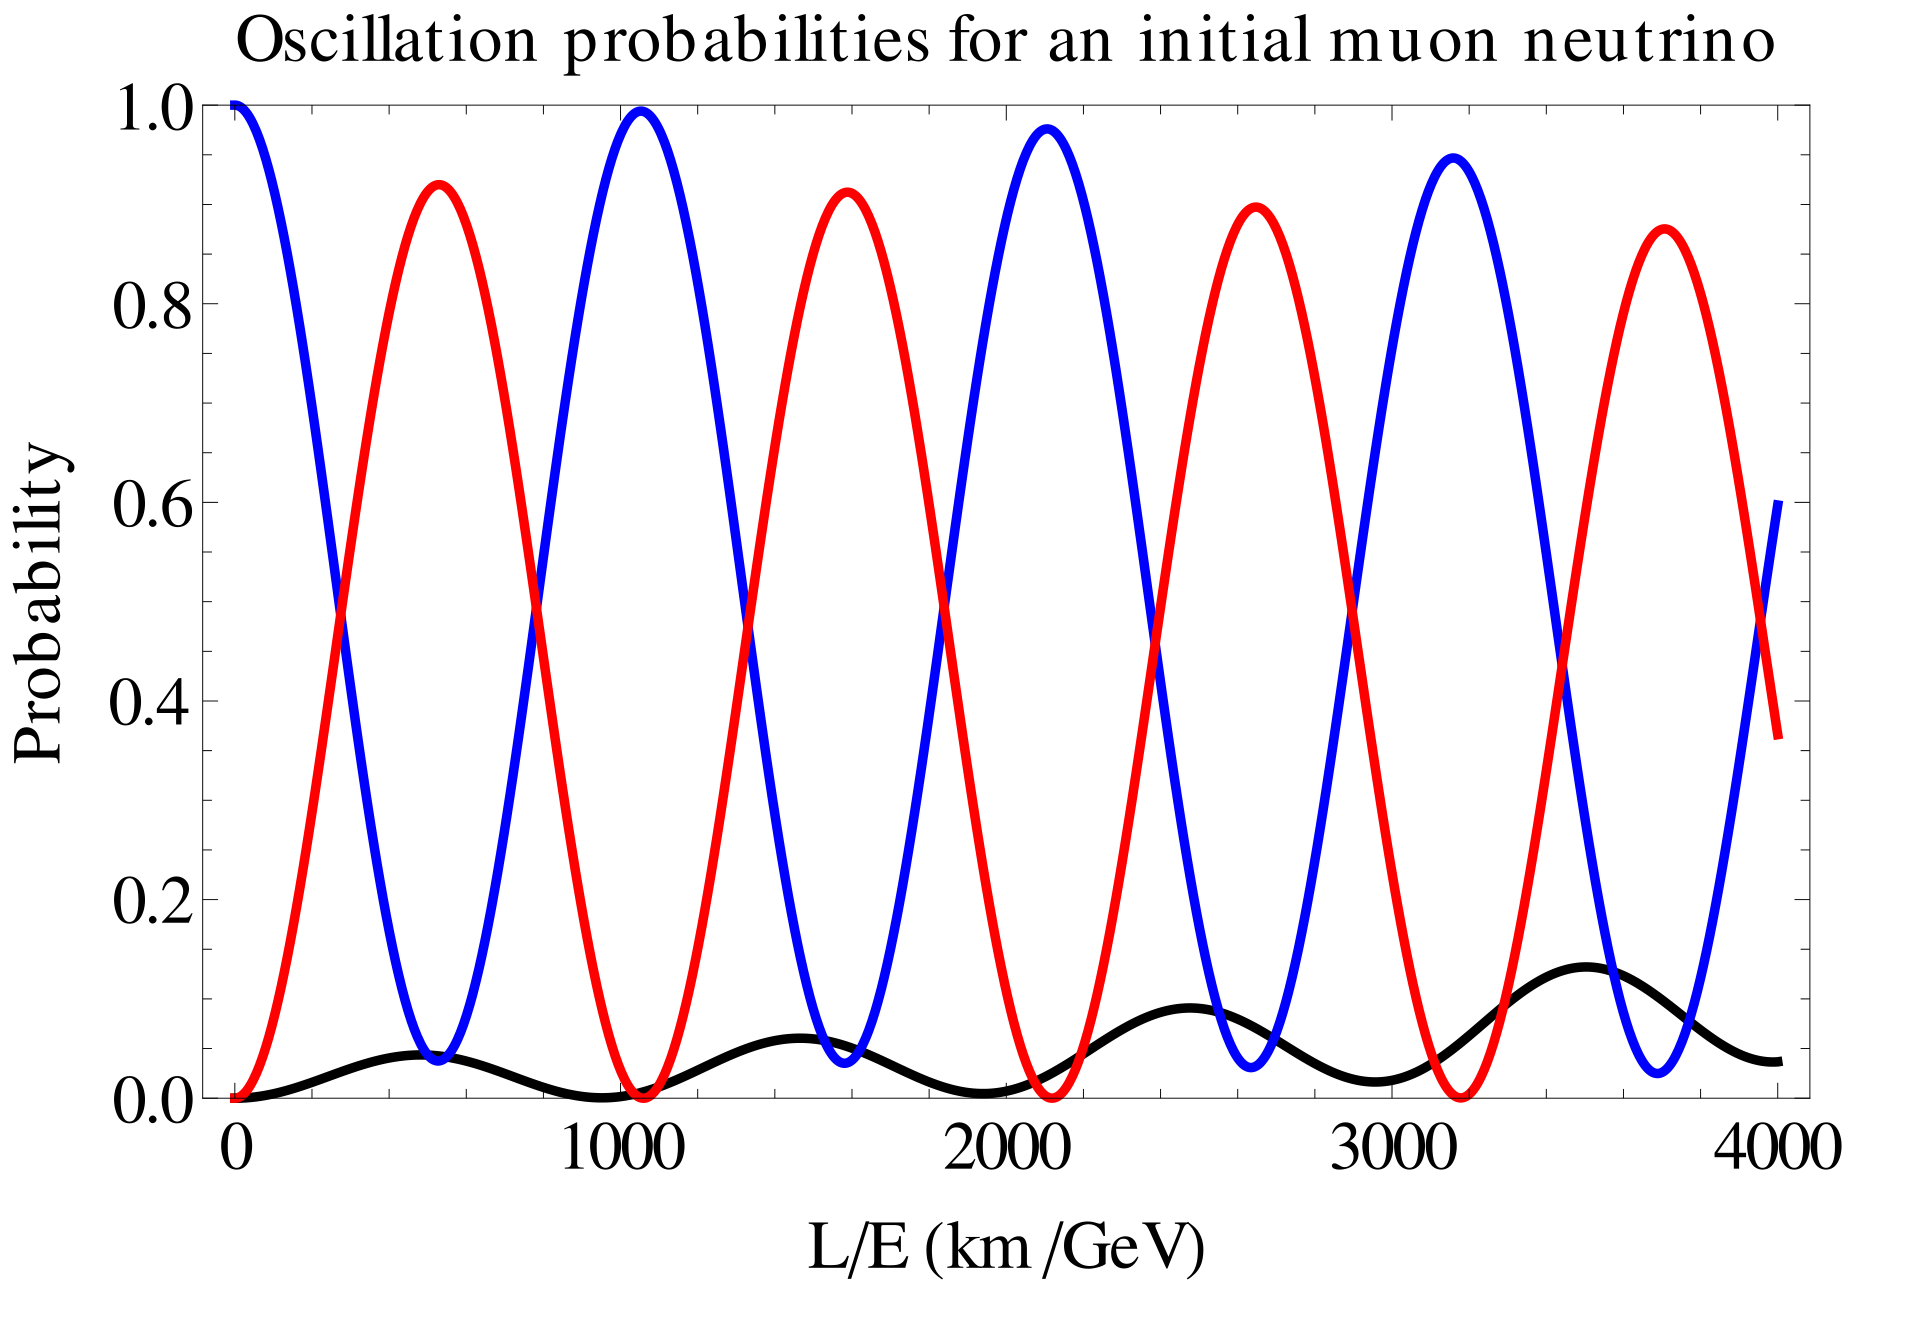
\includegraphics[width = 0.45\textwidth]{../figure/mu.png}  
            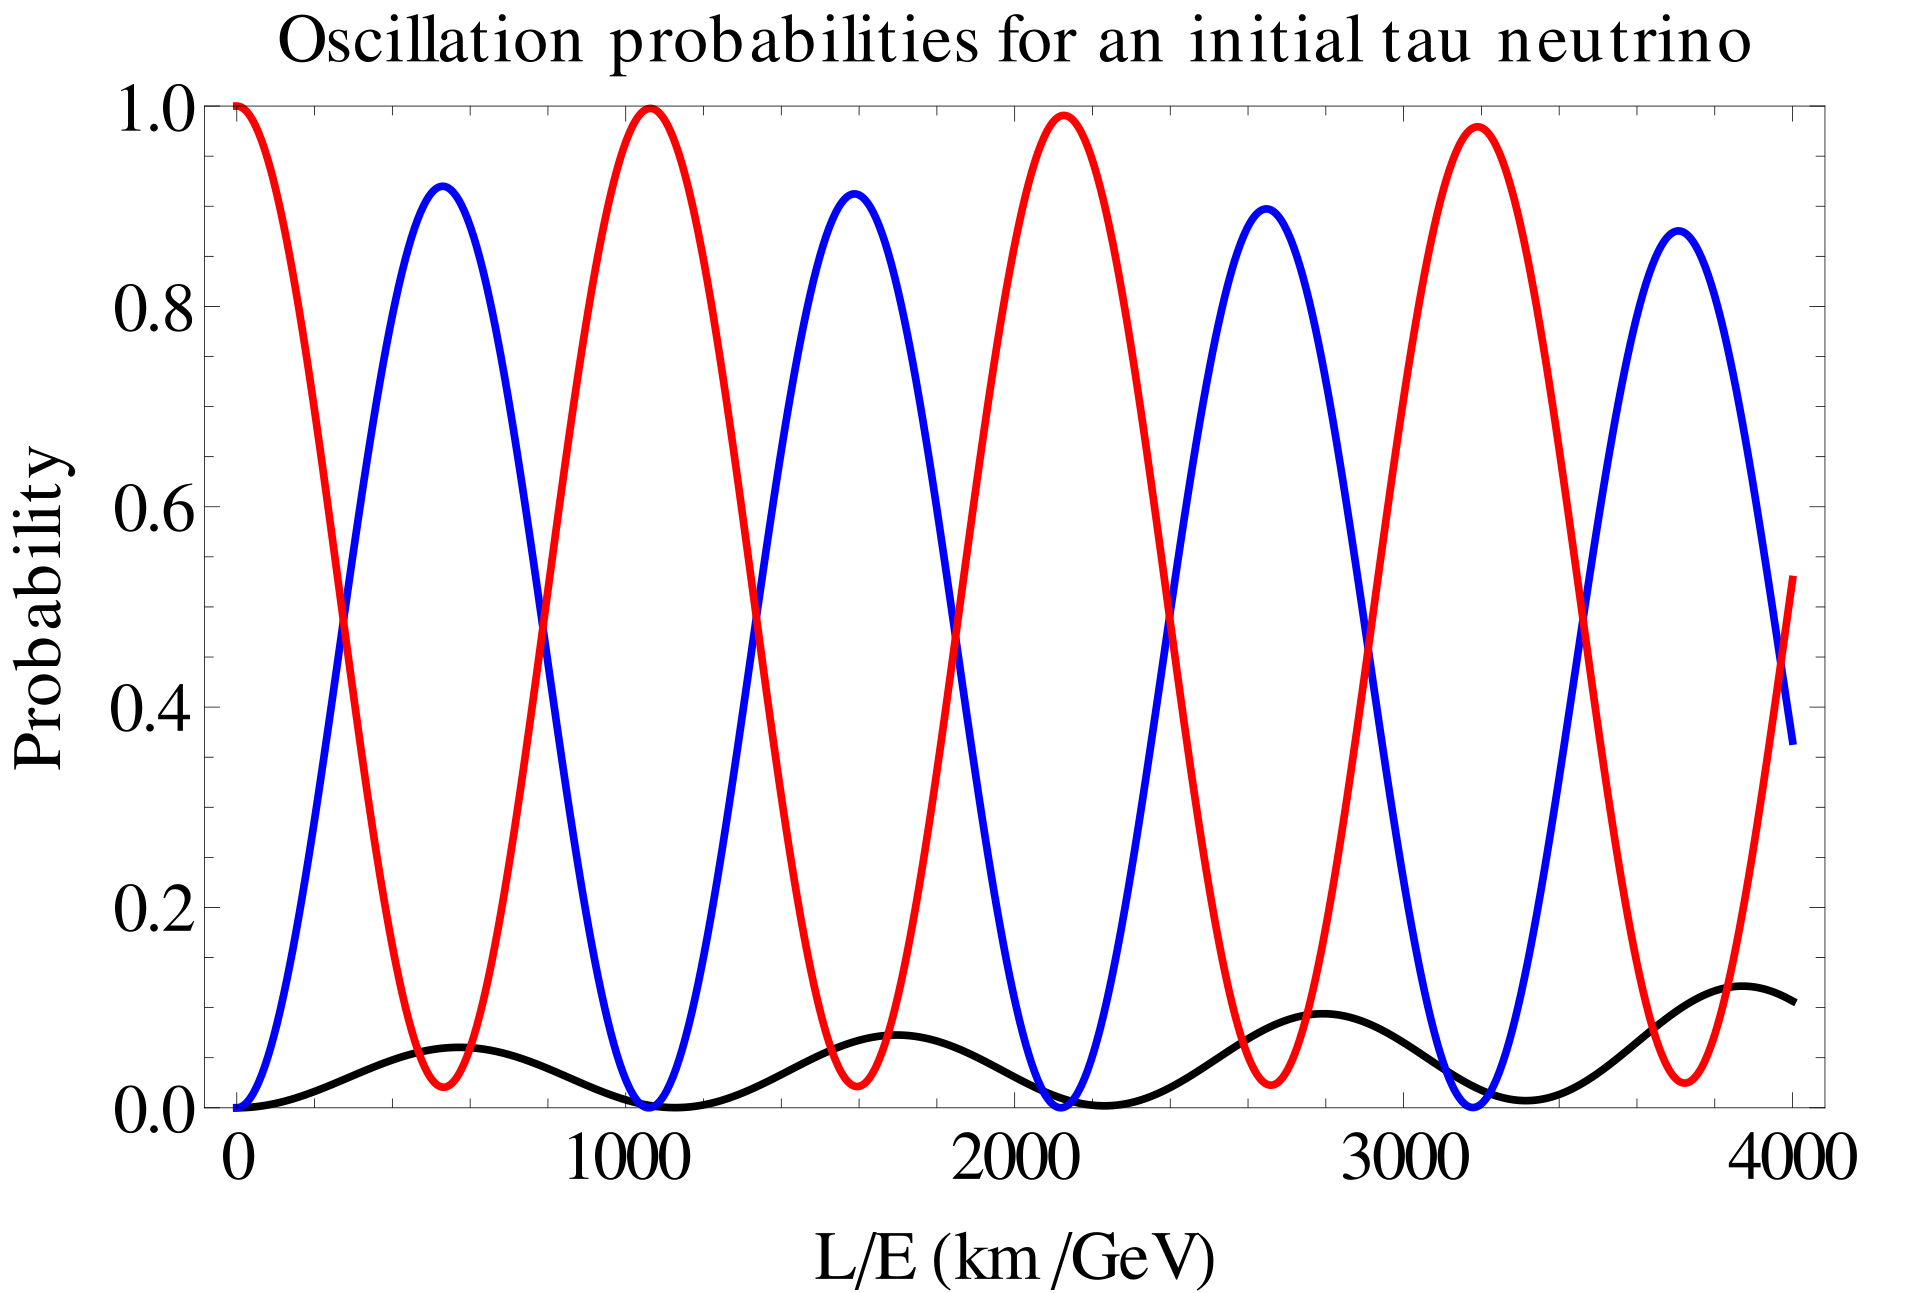
\includegraphics[width = 0.45\textwidth]{../figure/tau.png}  
            \caption{These three figures represent the probabilities in two flavors oscillations from the atmosphere. The top is the initial electron neutrino oscillating to others from the atmospheric neutrino source. The black line is the electron neutrino, the blue line is the muon neutrino, and the red line is for the tau neutrino; likewise, the middle is the initial muon neutrino, and the bottom is the initial tau neutrino. In this scenario, we find that electron neutrinos almost do not partake in the flavors exchange. \cite{wiki}}
            \label{NeuOsci}
        \end{figure}

\section{Super Kamiokonde}
    Super-Kamiokande is a 50 kton water Cherenkov detector instrumented with 11,146 photomultiplier tubes (PMTs) facing an inner 22.5 kton fiducial volume of ultrapure water located under Mount Ikeno near the city of Hida, Gifu Prefecture, Japan. \cite{SKinfo}

    \begin{figure}[H]
        \centering
        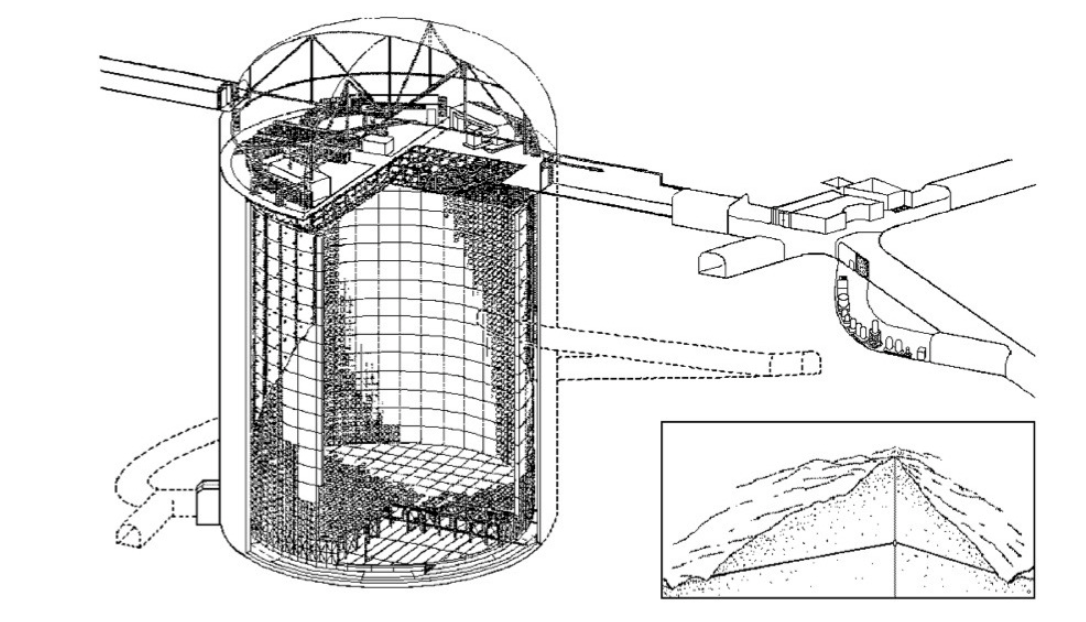
\includegraphics[width = 0.45\textwidth]{../figure/dect.png}
        \caption{Super Kamiokonde detector. \cite{dect}}
        \label{dect}
    \end{figure}

    In this report, we will show the Super-K experiment result in 1998 \cite{SKinfo}. According to the outcomes, the data is consistent at $90\%$ confidence level with the oscillation between muon neutrinos and tau neutrinos with $\sin^{2} 2\theta > 0.82$ and $5 \times 10^{-4} < \Delta m^{2} < 6 \times 10^{-3}\ [eV^{2}]$; however, these do not meet the best prediction of the expectations (Figure \ref{result1}). Therefore, I find other literature with the amendment of the effect of $\theta_{13}$ (brief theoretical introduction is in sec. I-ii), due to the time limit and the article length, I am not going to 
    expound on the detail mixing angle experiment data in this article. However, the data in 1998 \cite{SKinfo} and the new data in 2006 \cite{SKexp} are in Figure \ref{result1} and \ref{result2}. Lastly, owing to the discovery of neutrino oscillations which further shows that neutrinos have mass, in 2015, Takaaki Kajita, in Super-K awarded the Nobel prize.

\end{multicols}

\clearpage
\vspace*{\fill}
\begin{center}
    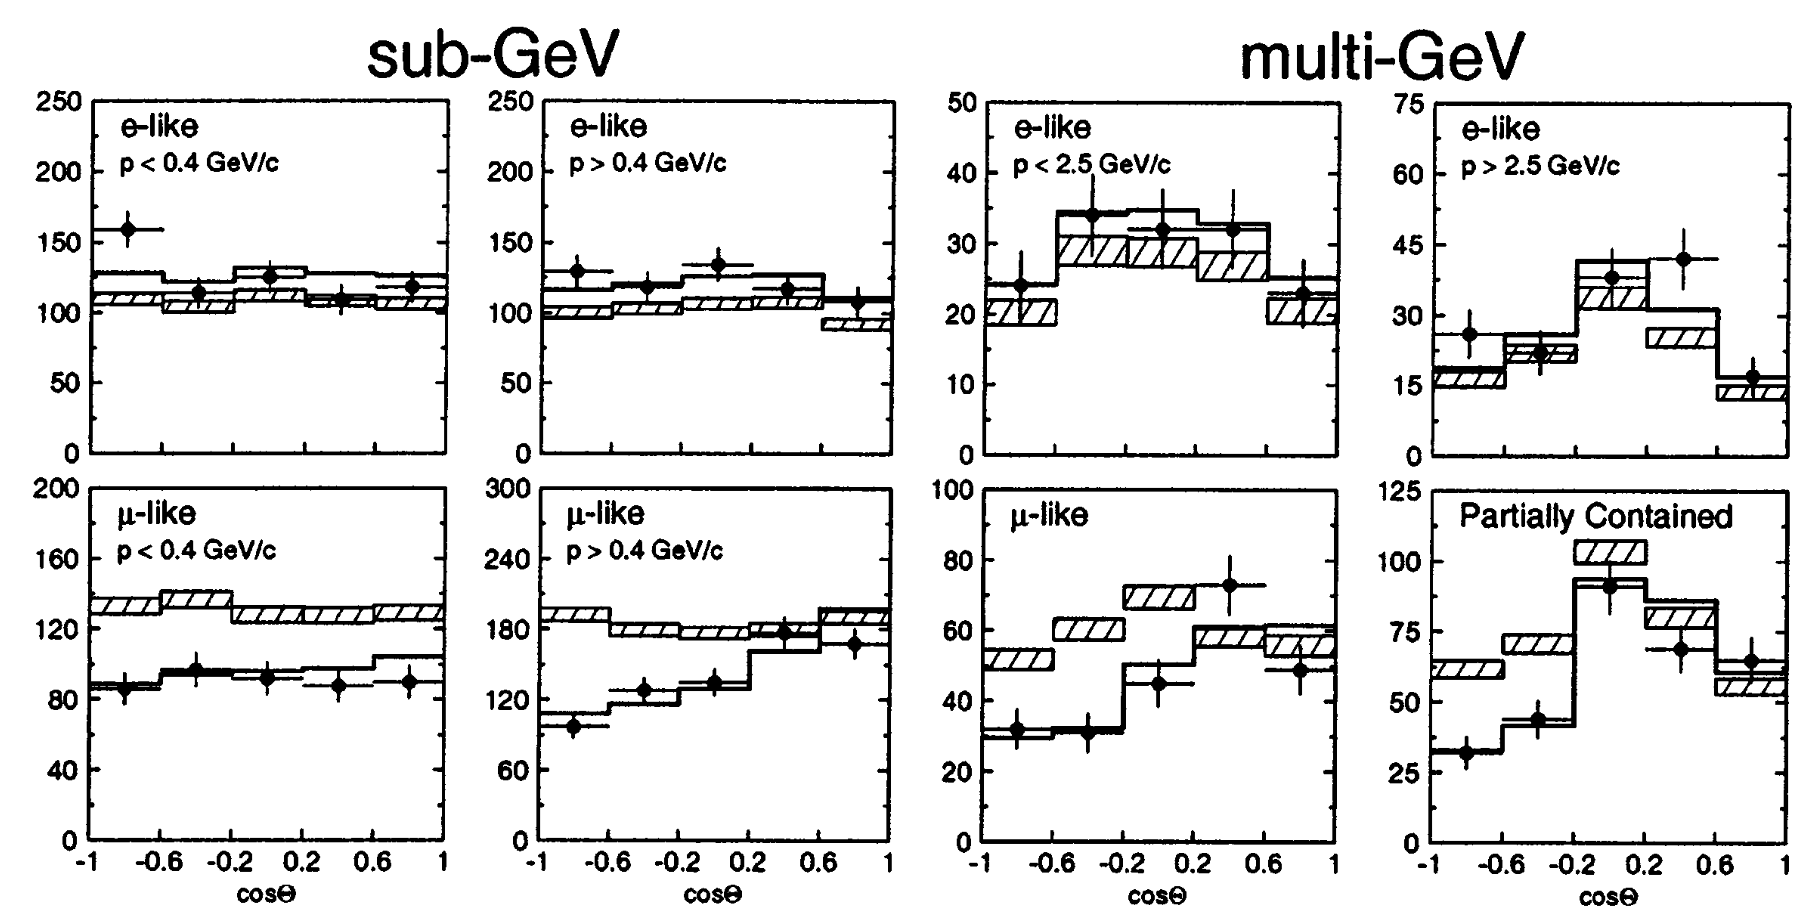
\includegraphics[width = 1\textwidth]{../figure/result1.png}
    \captionof{figure}{These are the figures that describe the zenith angle distribution of $\mu$-like or $e$-like events at sub-GeV(visible energy $E_{vis} < 1.33\ GeV$) and multi-GeV(visible energy $E_{vis} > 1.33\ GeV$), where the visible energy is the total energy assuming all Cherenkov light is from electromagnetic showers. The hatched region shows the Monte Carlo expectation for ``no oscillations normalized'' data with statistical errors. The bold line is the best-fit expectation for $\nu_{\mu} \leftrightarrow \nu_{\tau}$ oscillation with the overall flux normalization fitted as a free parameter. \cite{SKinfo} The up-going $\mu$-like events were manifestly smaller than the down-going ones; this is the obvious evidence for the neutrino oscillations. Besides, looking at $e$-like events, they fit our prediction which also meets our expectations for a slight (almost no) oscillation in the source of atmospheric neutrino oscillations \cite{dect}}
    \label{result1}
\end{center}
\vspace*{\fill}
\clearpage

    \begin{figure}[H]
        \centering
        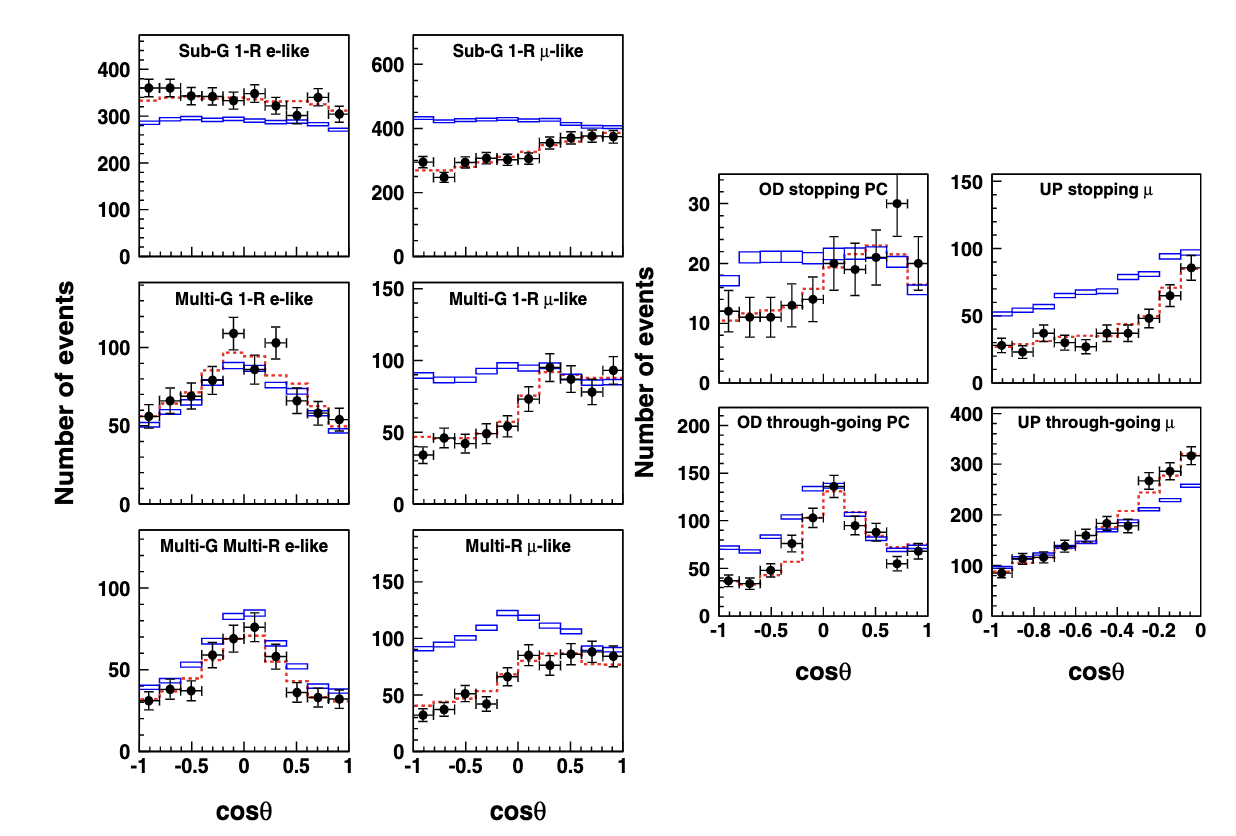
\includegraphics[width = 1\textwidth]{../figure/result2.png}
        \caption{These are the figures about the improvement of zenith angle distribution with the nonzeros $\theta_{13}$. The data are the filled circles with error bars; the best fit is the red dash line; the blue boxes are the mc data without neutrino oscillations. In contrast to these past experiments, the earth matter effect plays an important role in the analysis. \cite{SKexp}}
        \label{result2}
    \end{figure}

\begin{multicols}{2}

\begin{thebibliography}{1}

	%Each item starts with a \bibitem{} command and the details thereafter.
	
    \bibitem{SKexp} J. Hosaka et al. Physical Review D. Three flavor neutrino oscillation analysis of atmospheric neutrinos in Super-Kamiokande (2006).
    \bibitem{AtoNeu} Mclachlan Fukuei Thomas. The University of Tokyo, Japan. Study of the Oscillation of Neutrinos and Anti-Neutrinos and of Non-Standard Neutrino Interactions with the Atmospheric Data in Super-Kamiokande. (2015).
    \bibitem{SKinfo} Y. Fukuda et al. Physical Review Letters Evidence for Oscillation of Atmospheric Neutrinos (1998).
    \bibitem{dect}Y. Koshio. Universe. Review: Observation of Atmospheric Neutrinos (2020).
    \bibitem{Nobel}Takaaki Kajita. Discovery of Atmospheric Neutrino Oscillations. Institute for Cosmic Ray Research, The University of Tokyo, Japan. (2015)
    \bibitem{Fermilab} Neutrino Group. SLAC. Neutrino Oscillation \url{https://reurl.cc/ROQYoD} (2018)
    \bibitem{wiki} Wikipedia Contributors. Wikipedia. Neutrino oscillation (2022).
    
\end{thebibliography}

\end{multicols}


\end{document}